%%%%%%%%%%%%%%%%%%%%%%
%\begin{frame}{Idea}
%The pourpose of the ComTector algorithm is to find the communities in the given network.
%\vskip 0.5cm
%\begin{block}{\emph{Communitiy}}
%A \emph{community} is a subgraph of the given network characterised by a high number of intra-network connections and a low number of inter-network connections.
%\end{block}
%\vskip 0.5cm

%Individuals belonging to the same community are likely to have properties in common.

%\end{frame}

%%%%%%%%%%%%%%%%%%%%%%
\begin{frame}{Definitions}

\begin{description}
\vskip 0.7cm	
	\item[\emph{Definition 1}]: $S \subseteq V(G)$,$ \forall u , v \in S, u \neq v$, such that $(u,v) \in E$, then $S$ is a clique in $G$. If any other $S'$ is a \textbf{clique} and $S' \supseteq S$ iff $S' = S$, $S$ is a \textbf{maximal clique} of $G$.
\vskip 0.5cm	
	\item[\emph{Definition 2}]: For a given vertex $v$, $N(v) = \{ u | (v,u) \in E(G) \}$. We call $N(v)$ the set of all \textbf{neighbors} of $v$. Given a set $S \subseteq V(G)$, ${N|}_S = \bigcup N(v_i) - S$, $v_i \in S$, ${N|}_S$ is the set of all neighbors of $S$.
\vskip 0.5cm
	\item[\emph{Definition 3}]: Let $Com(G)$ be the set of all components in $G$. The giant component is denoted by $C_G$ and $M(C_G)$ is the set of all the maximal cliques in $C_G$. We use $V_M \subseteq V(G)$ to represent the set of all vertices  covered by $M(C_G)$.
\end{description}

\end{frame}

%%%%%%%%%%%%%%%%%%%%%%
\begin{frame}{Definitions}

\begin{description}
\vskip 0.7cm	
	\item[\emph{Definition 4}]: Let $P_0,P_1,...,P_{n-1}$ be the subgraph of $G$ such that $\forall P_i,P_j, V(P_i) \cap V(P_j) = \emptyset$, and $V(P_0) \cup , ... , V(P_{n-1}) = V(G)$. For any pair of $P_i$ and $P_j$, if $|E(P_i)| > |(N|_{P_i} \cap P_j)|$, $P_i$ is defined as a \textbf{community} of $G$.
\vskip 0.5cm	
	\item[\emph{Definition 5}]: Given vertex $v_i \in V_M$, define $C_i = \{S|S \in M(C_G), v_i \in S \}$ to be the set of all maximal cliques containing $v_i$, and $C$ the set of all $C_i$'s. $\forall C_i, C_j \in C$, if $ \frac{| C_i \cap C_j |}{|C_j|} \geq f$, which is a threshold to describe the extent to which $C_i$ overlaps with $C_j$, we call $C_j$ is contained in $C_i$, denoted by $C_j < C_i$. If $C_i$ is not contained by any other element in $C$, $C_i$ is called the \textbf{kernel} of $G$ and $v_i$ is the \textbf{center} of $C_i$
\end{description}

\end{frame}

%%%%%%%%%%%%%%%%%%%%%%
%\begin{frame}{Definitions}

%\begin{description}
%\vskip 0.7cm	
%	\item[\emph{Definition 6}]:  Let $K$ be the set of all kernels in $G$. $V_K = \{ v_i | v_i \in k_j, k_j \in K\}$ is the set of all %vertices covered by $K$ and $I_K = \bigcup(k_i \cap k_j), k_i, k_j \in K, i \neq j$ is the union of all the vertices that any pair of %elements in $K$ has in common.
%\end{description}

%\end{frame}

%%%%%%%%%%%%%%%%%%%%%%
\begin{frame}{Structure}
\vskip 0.7cm
The following is the algorithm of the structure of ComTector presented in the paper at the end of the relative section.
\begin{center}
	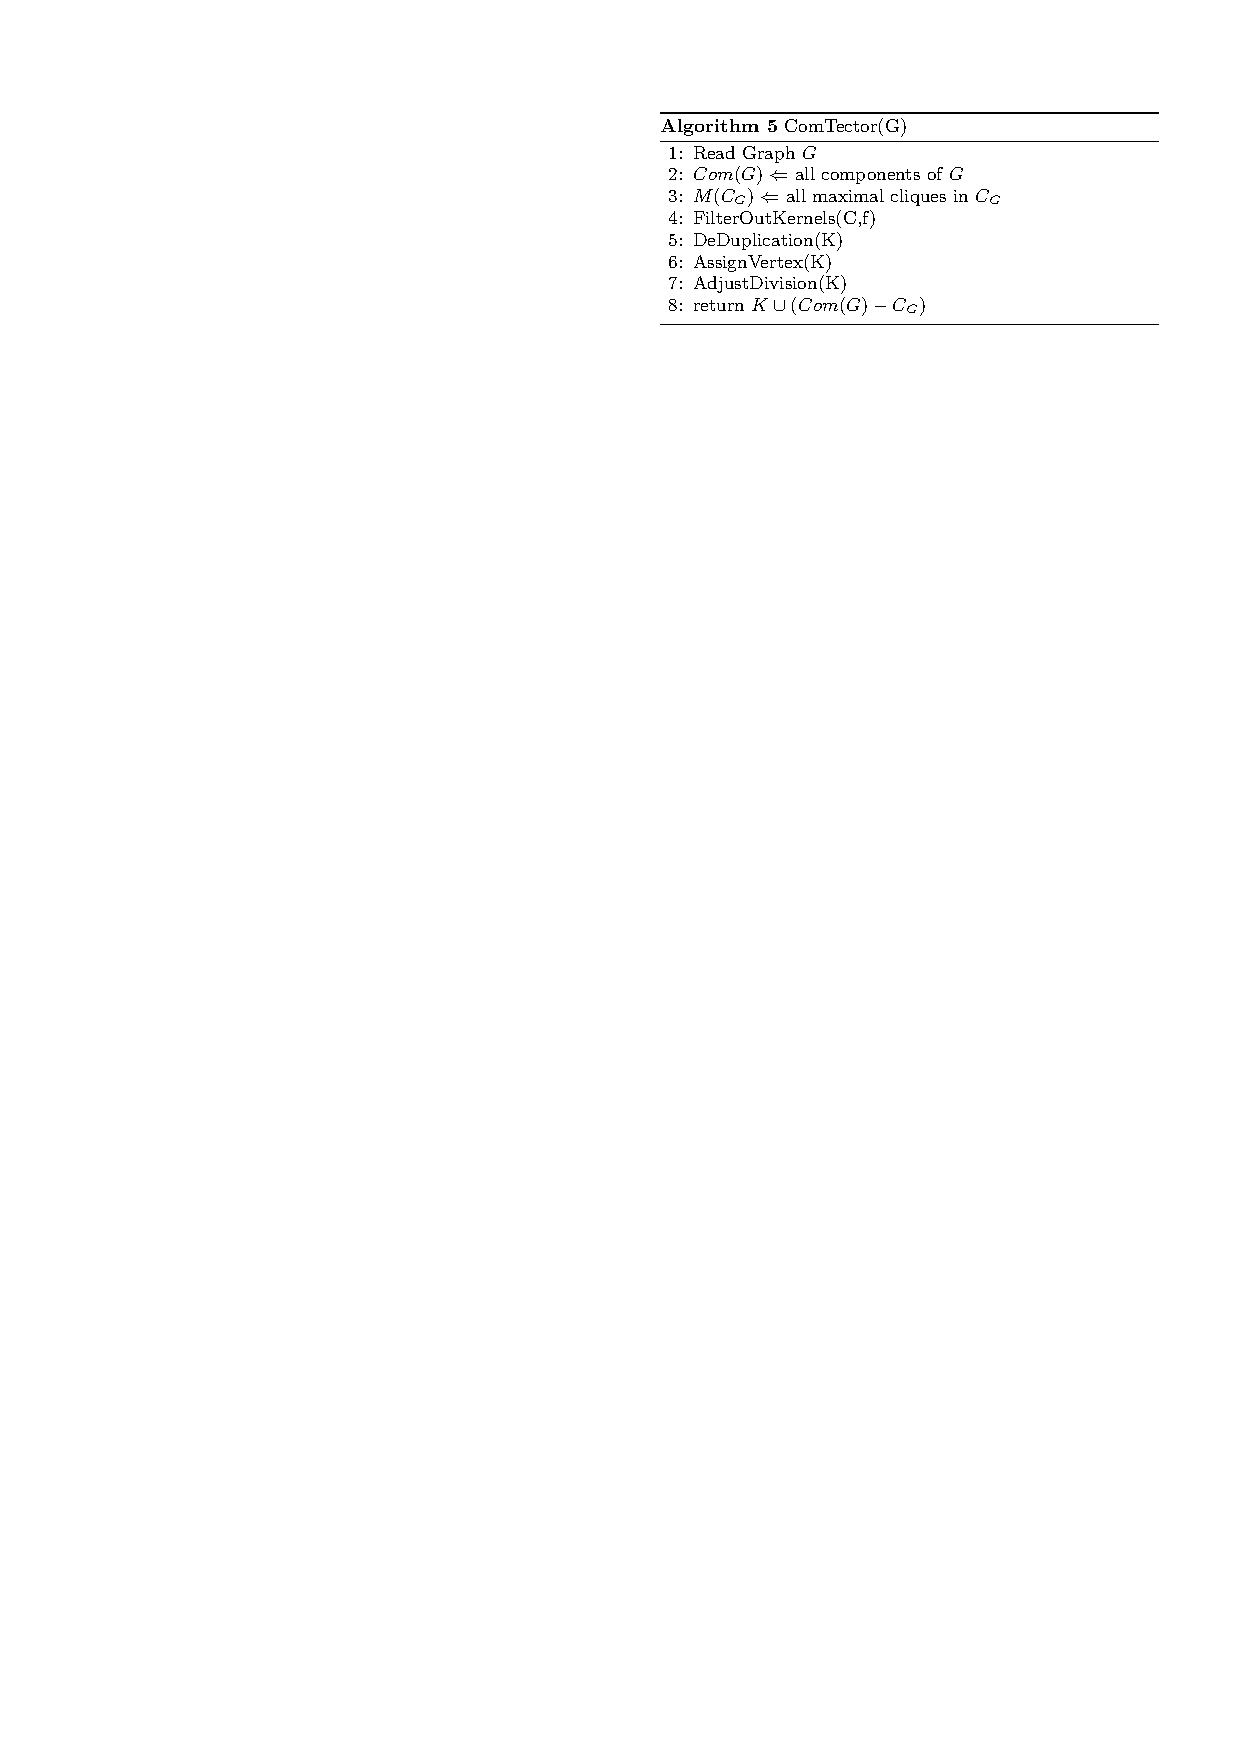
\includegraphics[height=5cm]{images/comTectorStructure.pdf}
\end{center}

\end{frame}

%%%%%%%%%%%%%%%%%%%%%%
%\begin{frame}{First steps}
%\vskip 0.5cm
%Loading the graph and finding all the components of the network is quite simple because ComTector operates on undirected network without self loops that are typical of social networks. 
%\begin{block}{Component}
%In graph theory, a \textbf{connected component} (or just component) of an undirected graph is a subgraph in which any two vertices are connected to each other by paths, and which is connected to no additional vertices in the supergraph. \footnote{From Wikipedia, the free encyclopedia}
%\end{block}

%\end{frame}

%%%%%%%%%%%%%%%%%%%%%%
%\begin{frame}{Maximal cliques}
%\vskip 0.5cm
%the enumeration of all maximal cliques in the giant component by using \emph{Peamc} \footnote{Peamc is a parallel algorithm that splits the computation of the cliques in $N$ nodes. It is not analized in the paper nor in these slides, for further informations see: \\
%\emph{N. Du, B. Wu, and B. Wang. \\A parallel algorithm for enumerating all maximal cliques in complex networks. \\In The 6th ICDM2006 Mining Complex Data \\Workshop, pages 320–324. IEEE CS, December 2006.}} will cost:
%$$ O(\Delta \times M_C \times Tri^2)$$

%Where:

%\begin{description}
%	\item[$\Delta$]: is the maximal degree of $G$
%	\item[$M_C$]: is the size of the maximum cliques
%	\item[$Tri$]: is the number of all triangles in $G$
%\end{description}

%\end{frame}

%%%%%%%%%%%%%%%%%%%%%%
%\begin{frame}{Kernel generation}
%\vskip 0.5cm
%After we have found the maximal cliques, we arrange them in $C_i$s.
%\begin{center}
%	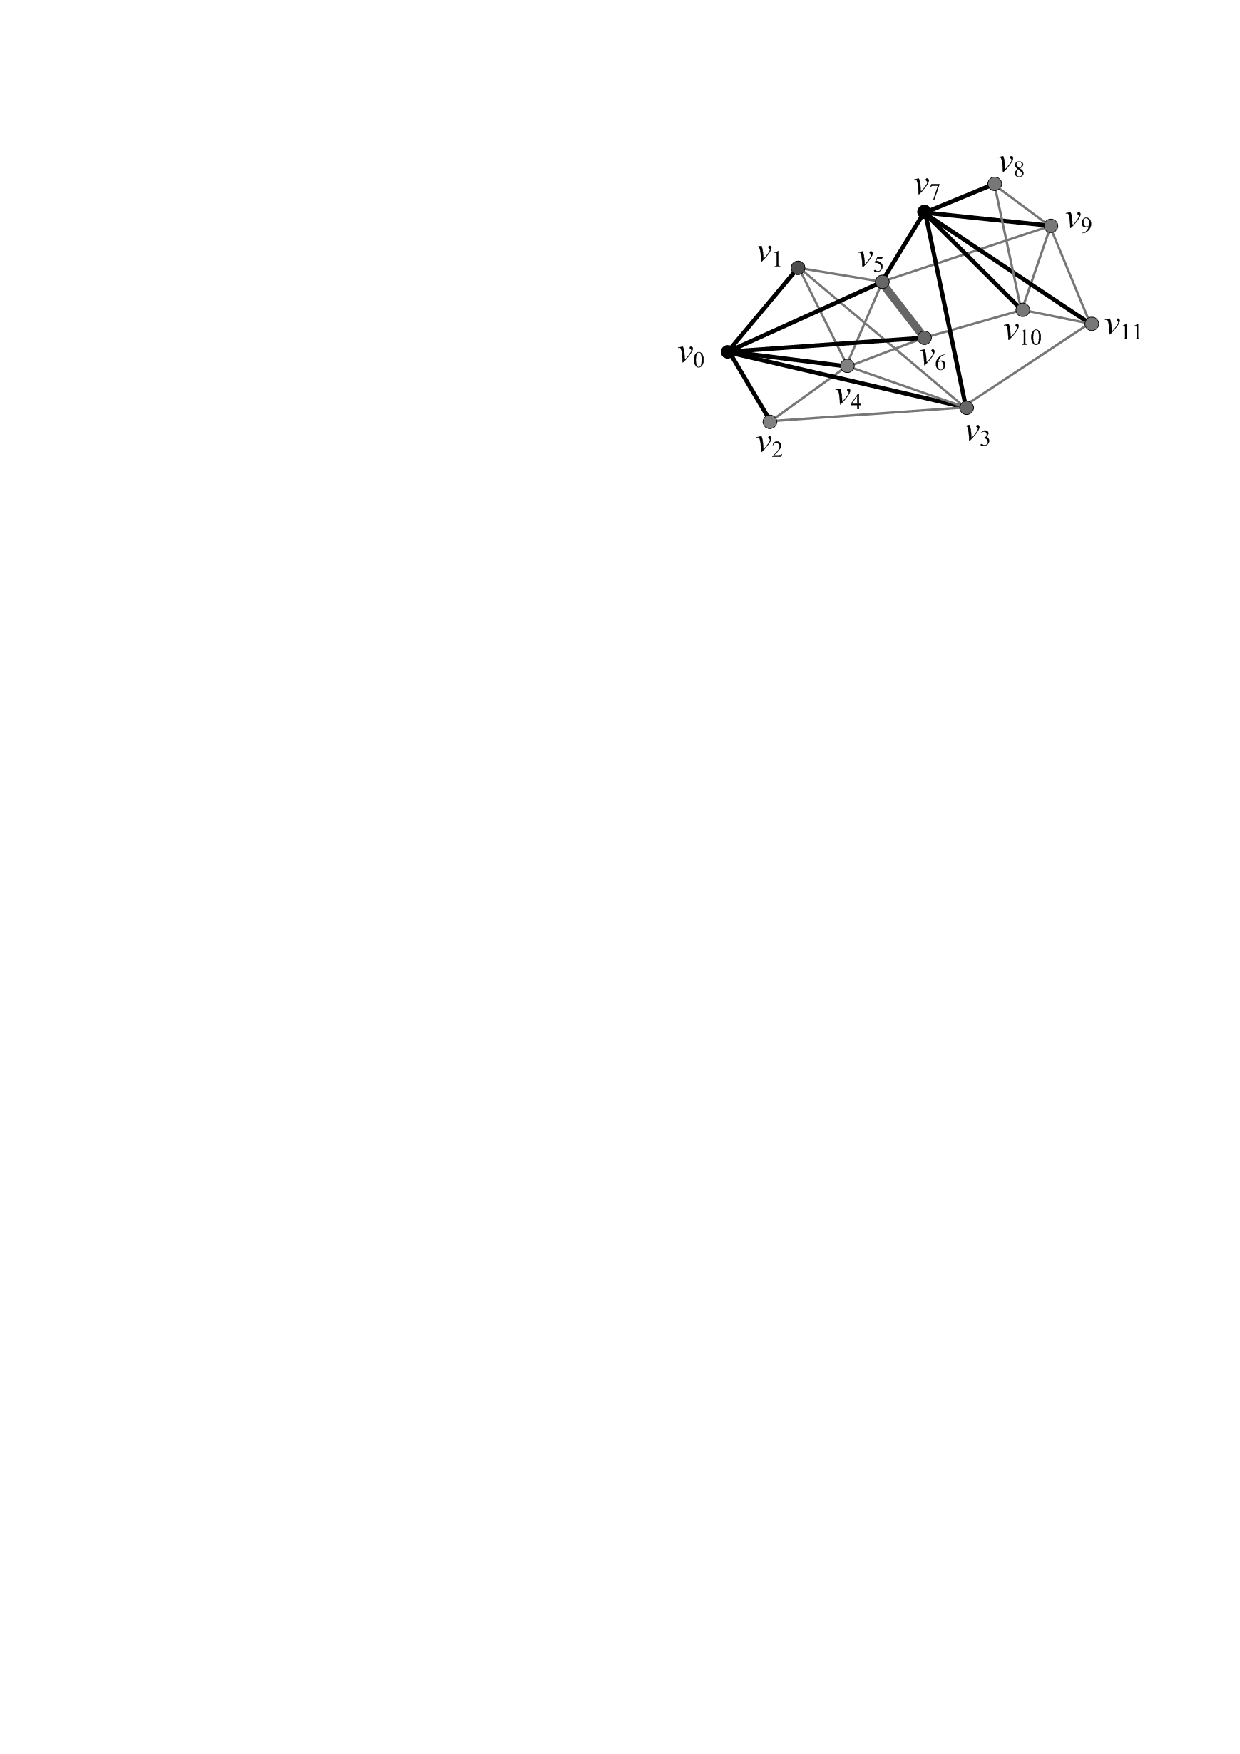
\includegraphics[height=4cm]{images/sampleNet.pdf}
%\end{center}
%Example:

%$C_0 = \{ \{v_0,v_1,v_4,v_5\}, \{v_0,v_1,v_3,v_4\}, \{v_0,v_2,v_3,v_4\}, \{v_0, v_4, v_5 , v_6\}\}$ with $v_0$ as center.

%$C_1 = \{ \{v_0,v_1,v_4,v_5\}, \{v_0,v_1,v_3,v_4\}\}$ with $v_1$ as center.

%\end{frame}

%%%%%%%%%%%%%%%%%%%%%%
\begin{frame}{Filter out kernels}
\vskip 0.5cm
Now we generate the kernel $K$ as shown in the algorithm.
\begin{center}
	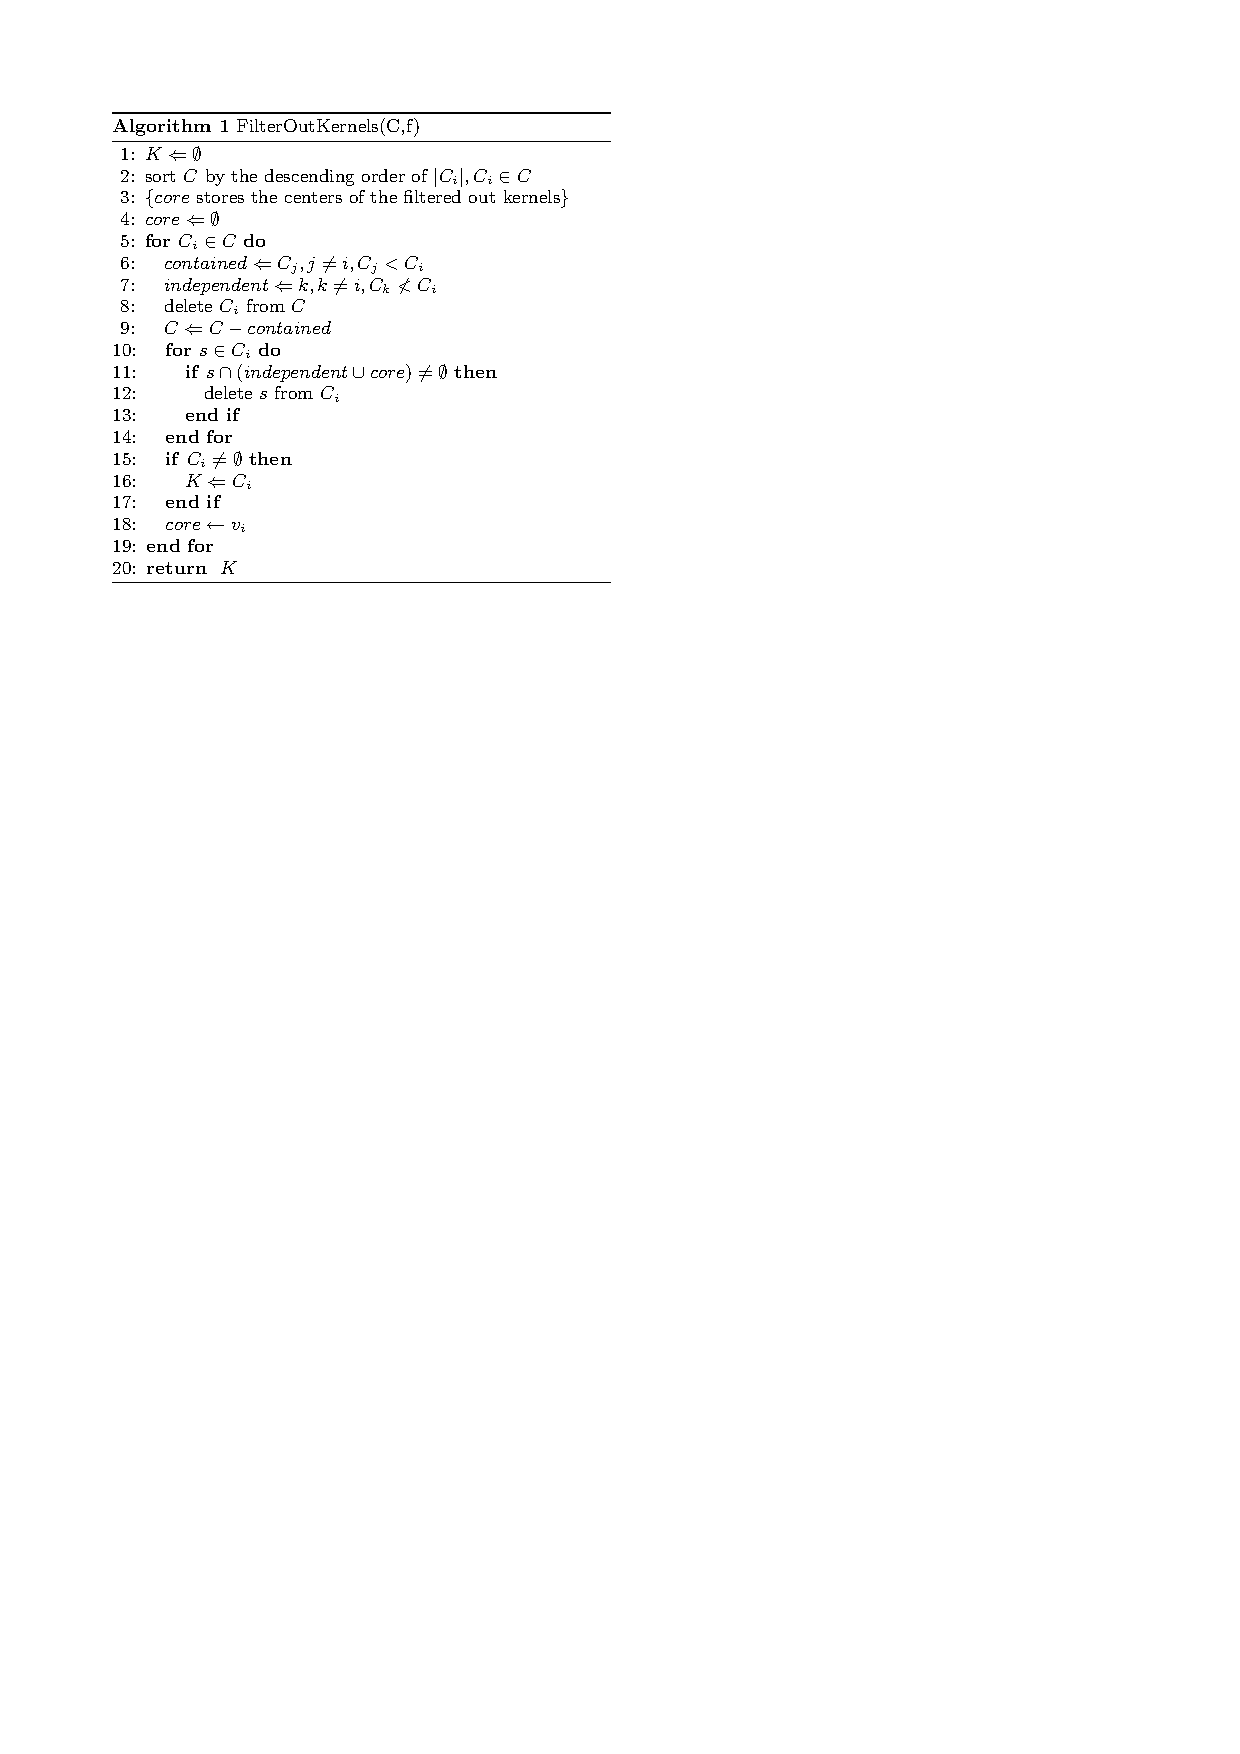
\includegraphics[height=7.1cm]{images/filterOutKernels.pdf}
\end{center}

\end{frame}

%%%%%%%%%%%%%%%%%%%%%%
%\begin{frame}{Filter out kernels}
%\vskip 0.5cm
%Recall:
%\begin{description}
%\item[\emph{Definition 5}]: Given vertex $v_i \in V_M$, define $C_i = \{S|S \in M(C_G), v_i \in S \}$ to be the set of all maximal cliques containing $v_i$, and $C$ the set of all $C_i$'s. $\forall C_i, C_j \in C$, if $ \frac{| C_i \cap C_j |}{|C_j|} \geq f$, which is a threshold to describe the extent to which $C_i$ overlaps with $C_j$, we call $C_j$ is contained in $C_i$, denoted by $C_j < C_i$. If $C_i$ is not contained by any other element in $C$, $C_i$ is called the \textbf{kernel} of $G$ and $v_i$ is the \textbf{center} of $C_i$
%\end{description}

%\vskip 0.5cm

%{\textcolor{green!40!black}{\fontsize{18}{20}\textbf{How can we choose $f$?}}}

%\end{frame}


%%%%%%%%%%%%%%%%%%%%%%
%\begin{frame}{Parameter tuning}
%\begin{center}
%	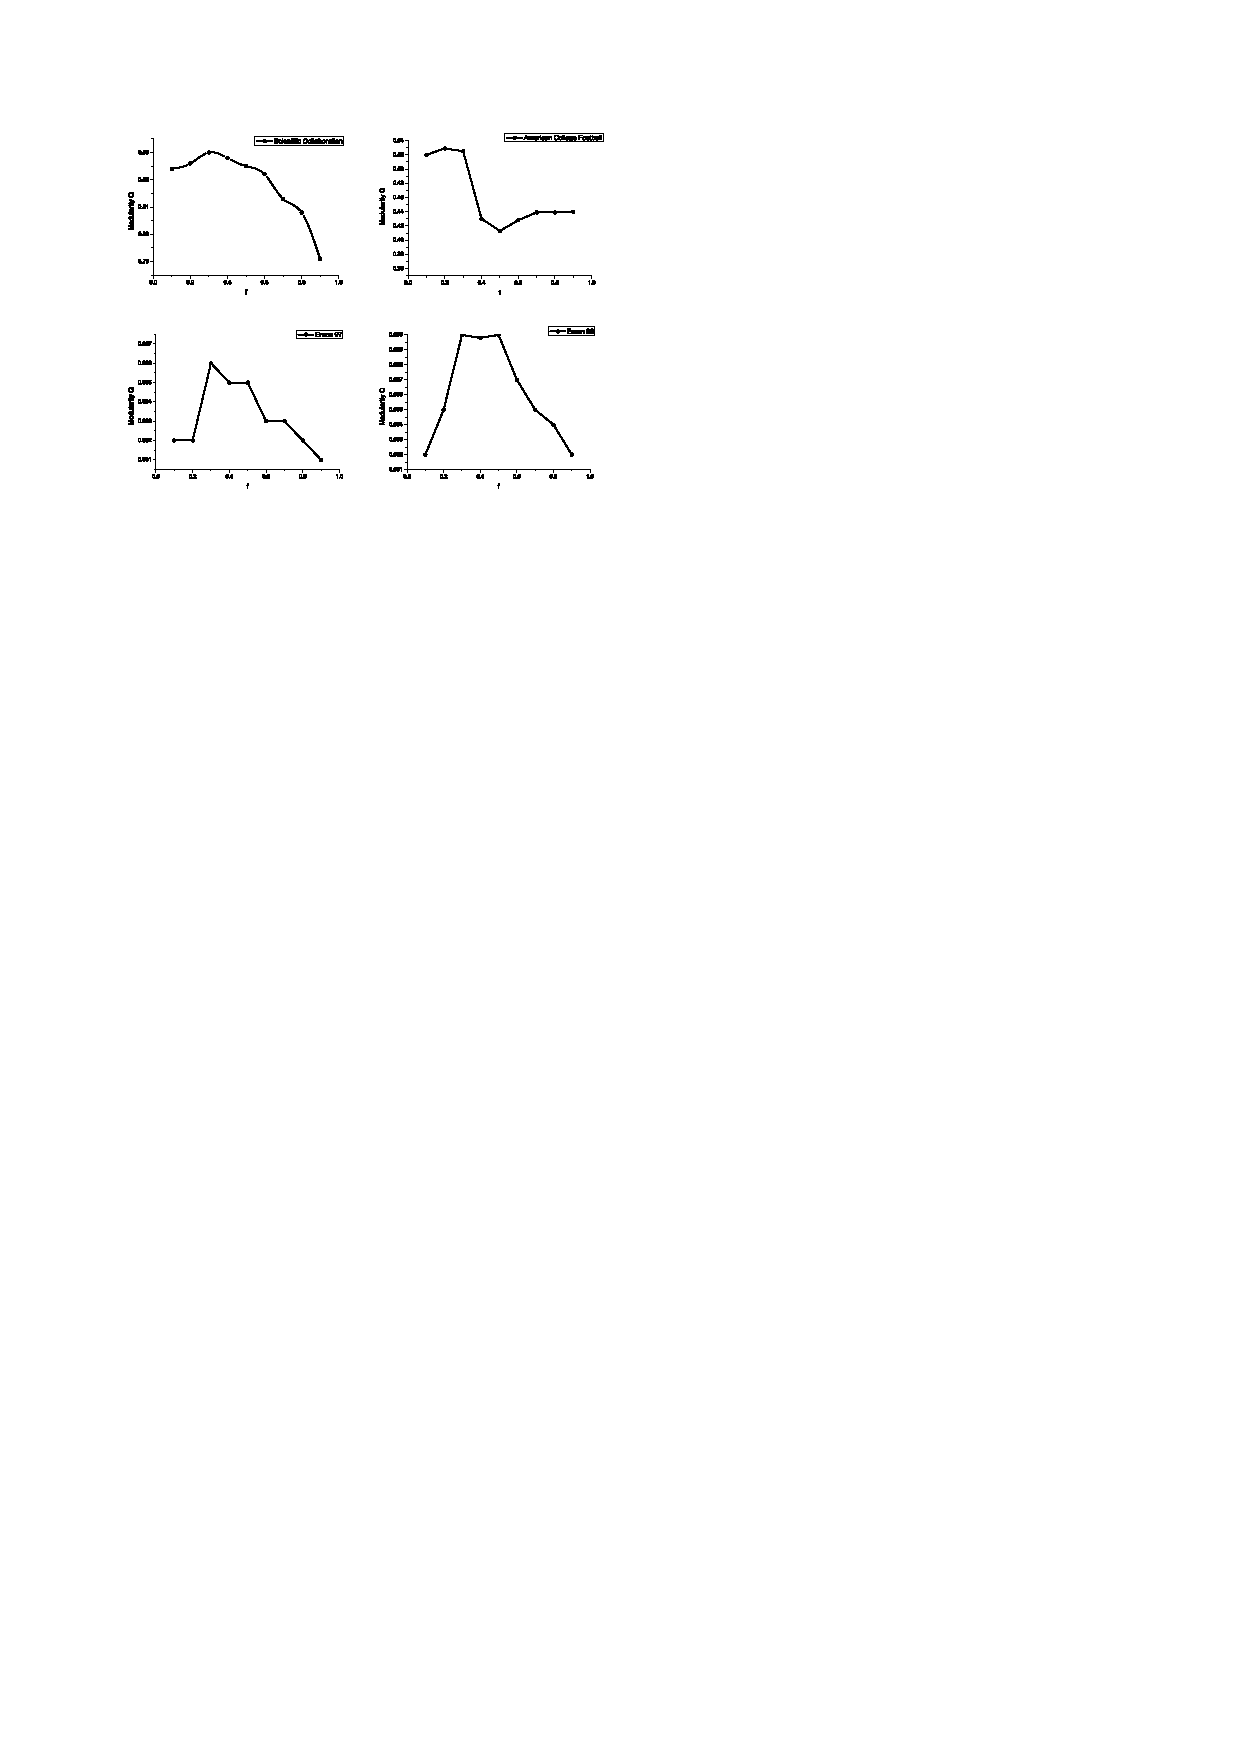
\includegraphics[height=6.2cm]{images/fChoice.pdf}
%\end{center}
%The authors suggest $f \in (0.3 , 0.5)$ as experimental result.

%\end{frame}

%%%%%%%%%%%%%%%%%%%%%%
%\begin{frame}{Kernel generation}
%\begin{center}
%	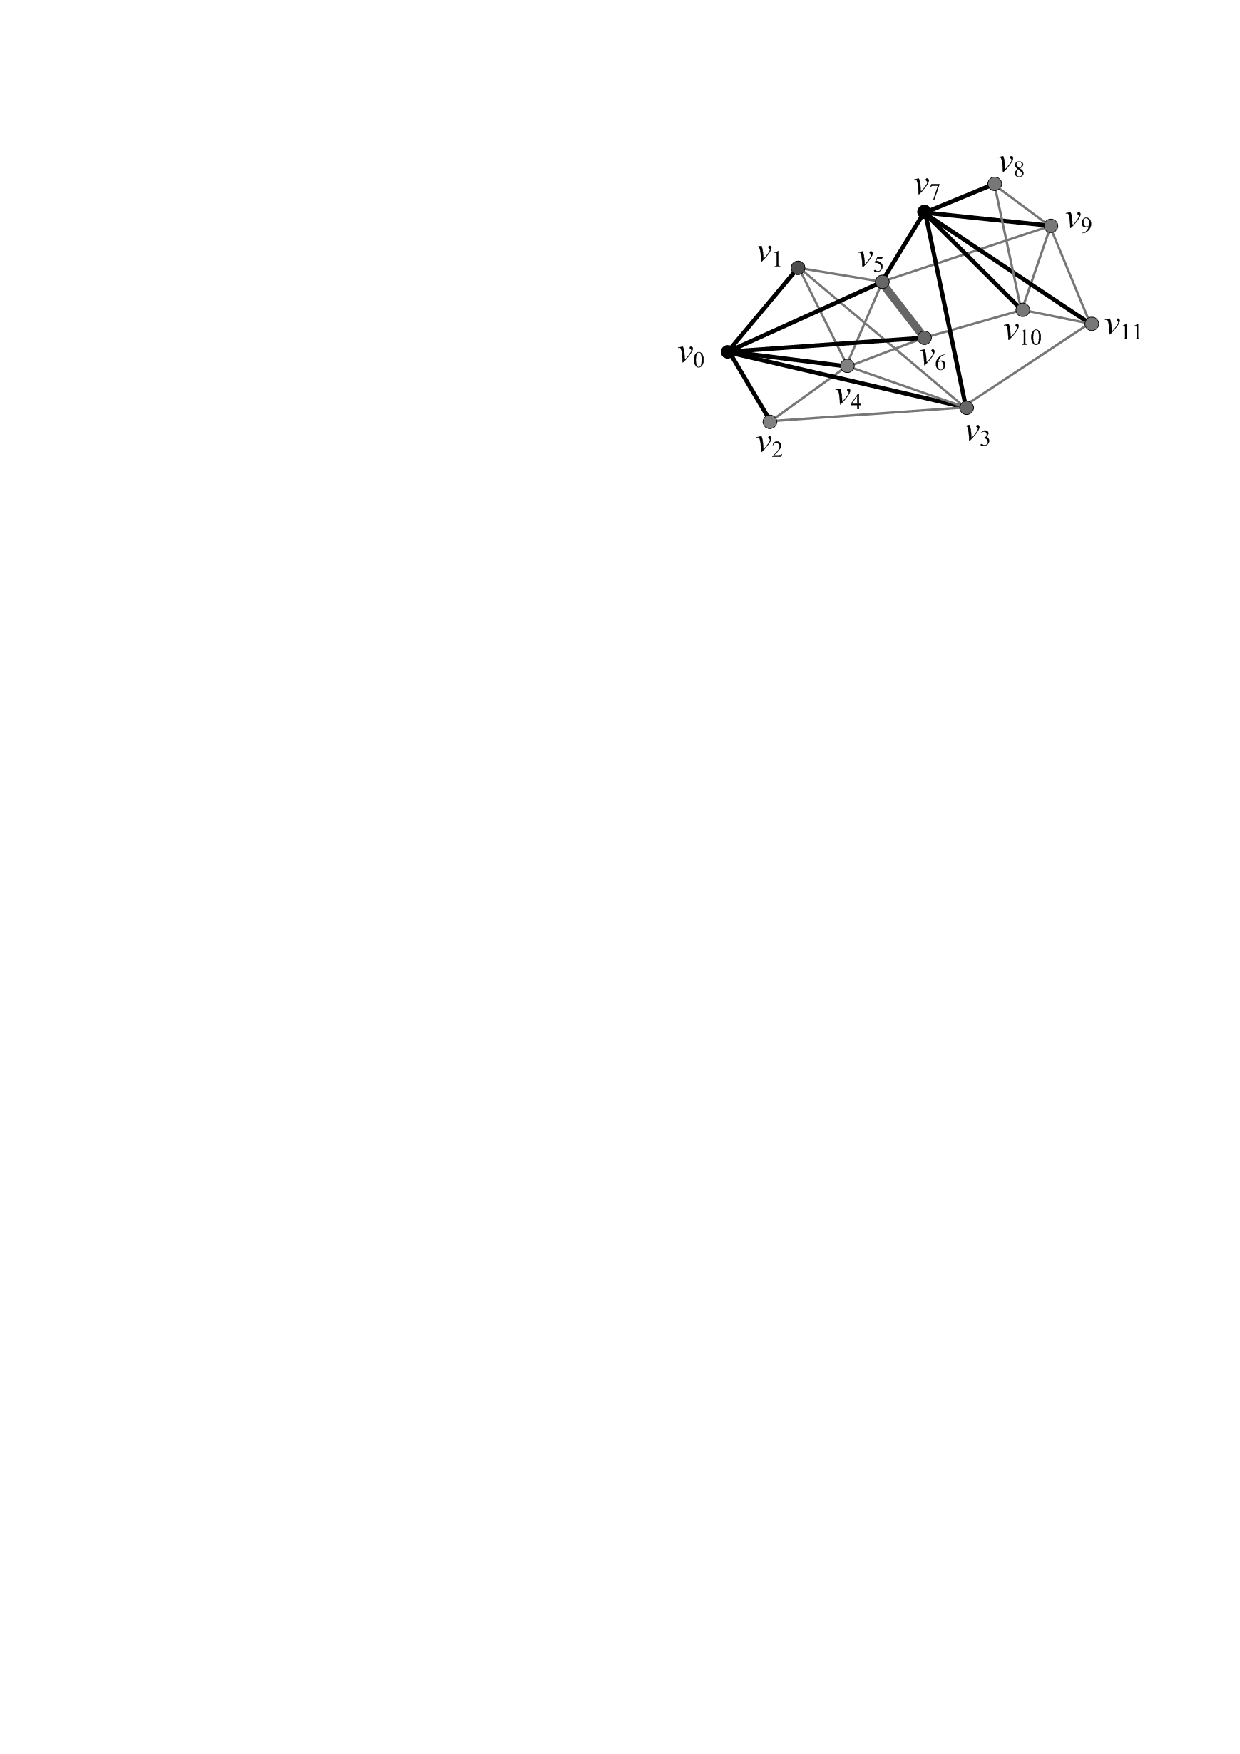
\includegraphics[height=3.7cm]{images/sampleNet.pdf}
%\end{center}

%The temporary kernel of the above network is the following:
%$$K = \{C_0, C_7\}$$
%Where:
%$$C_0 = \{ \{v_0,v_1,v_4,v_5\}, \{v_0,v_1,v_3,v_4\}, \{v_0,v_2,v_3,v_4\}, \{v_0, v_4, v_5 , v_6\}\} $$
%$$C_7 = \{\{v_7,v_8,v_9,v_{10}\}, \{v_7,v_9,v_{10},v_{11}\}\}$$
 
%\end{frame}

%%%%%%%%%%%%%%%%%%%%%%
\begin{frame}{DeDuplication}
\vskip 0.8cm
Now we have to choose only one kernel for those vertices that belong to multiple kernels.
\begin{center}
	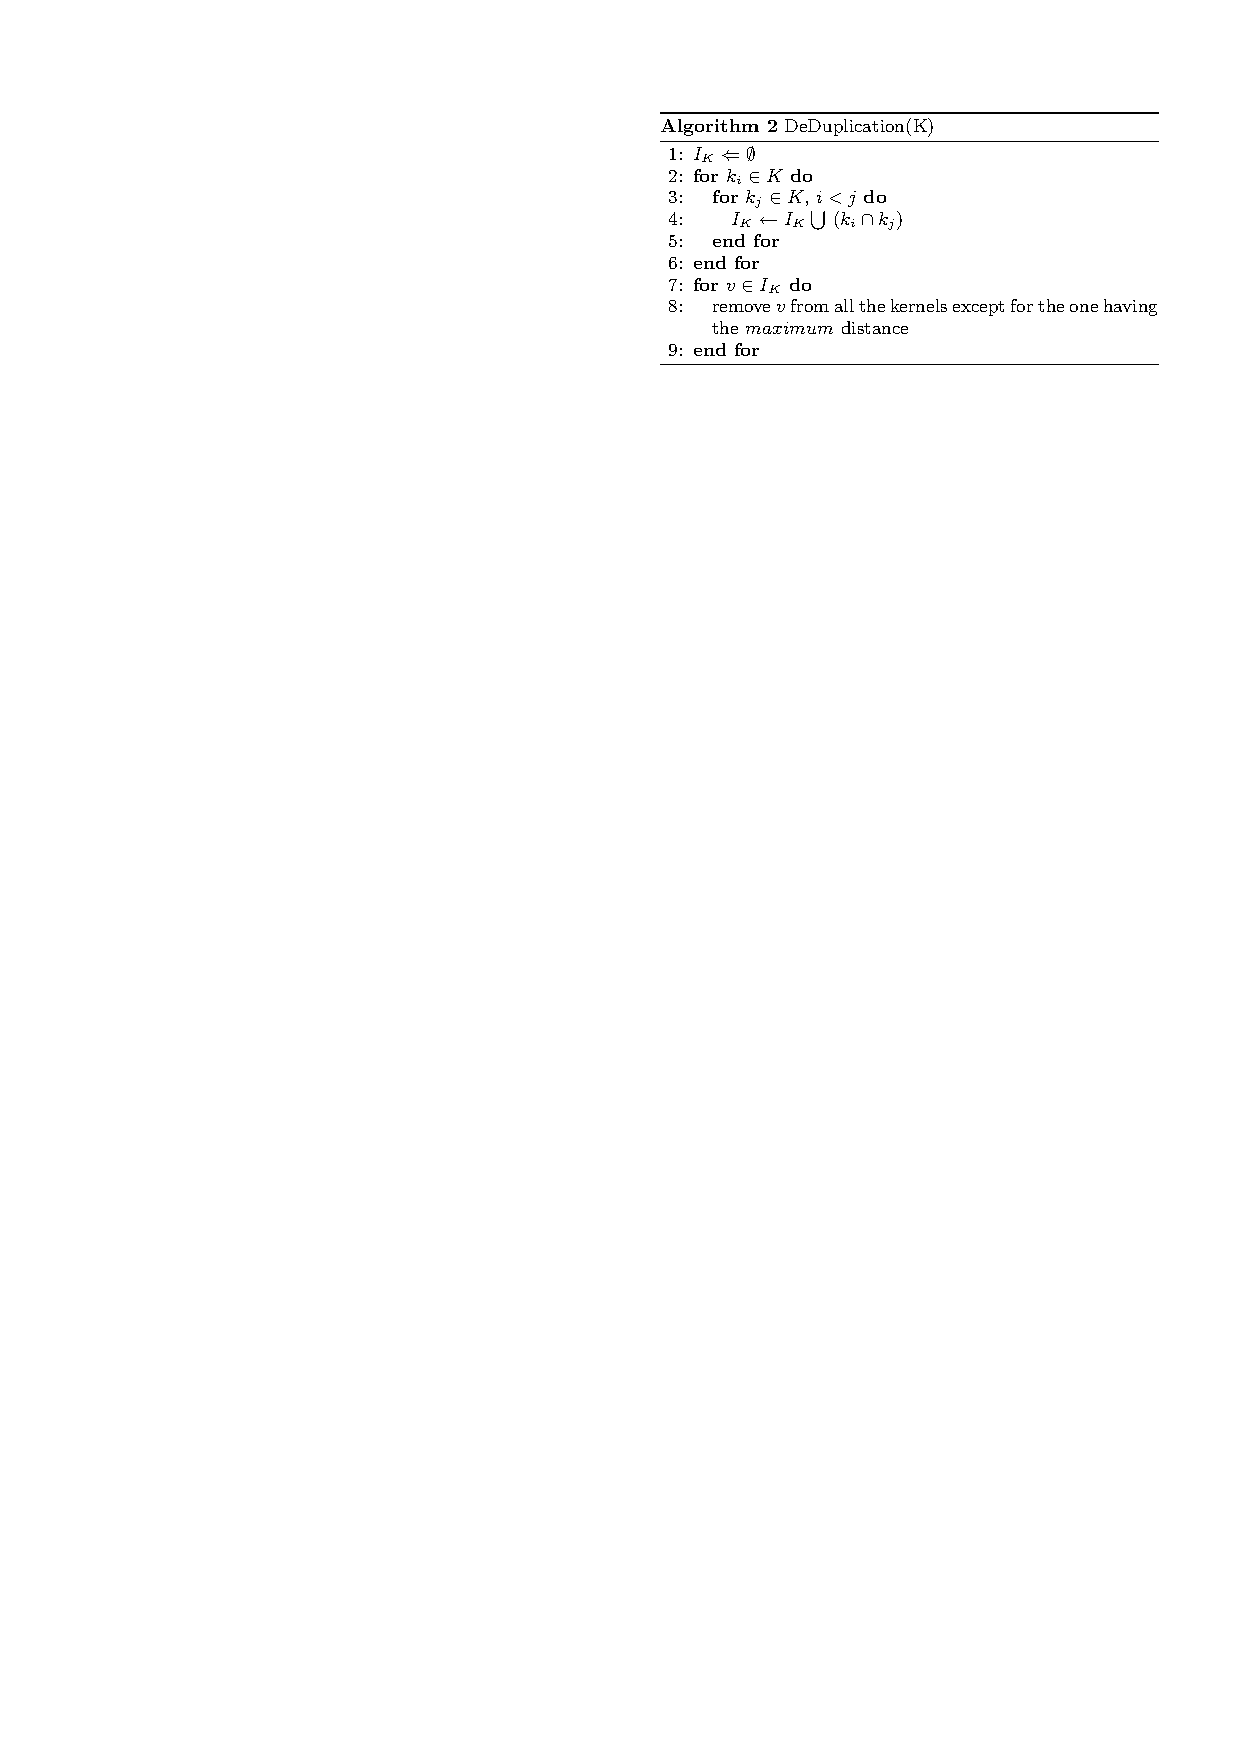
\includegraphics[height=5.5cm]{images/deduplication.pdf}
\end{center}
\end{frame}

%%%%%%%%%%%%%%%%%%%%%%
\begin{frame}{Assign vertex}
\vskip 0.9cm
Next step is to assign to the closest kernel all the remaining vertices.
\begin{center}
	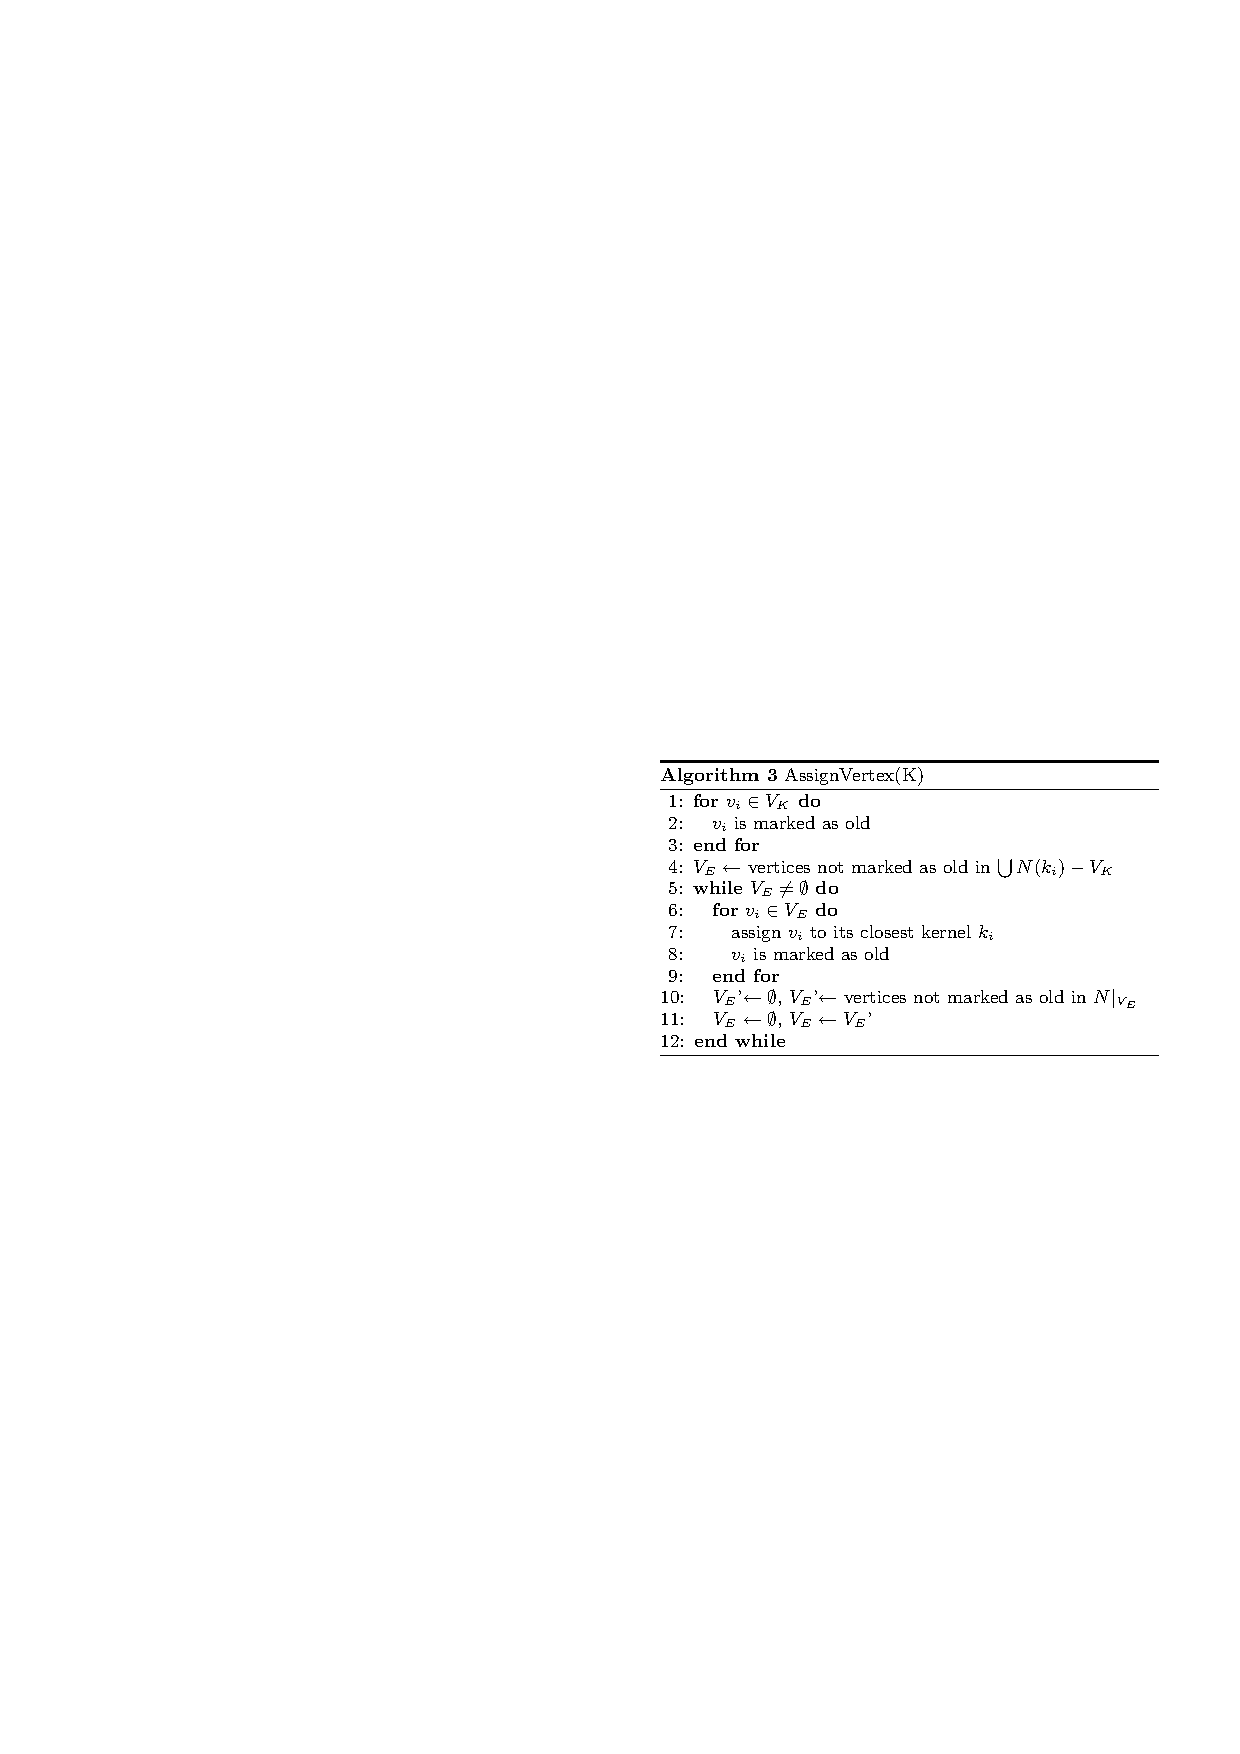
\includegraphics[height=6.3cm]{images/assignVertices.pdf}
\end{center}
\end{frame}

%%%%%%%%%%%%%%%%%%%%%%
%\begin{frame}{Modularity optimization}
%\vskip 0.7cm
%Now we have to agglomerate partitions in order to increase the \emph{Network Modularity Q}.
%\vskip 0.5cm
%$E = [ e _{ij}]$ is $p \times p$ symmetric matrix.
%\vskip 0.5cm
%$e_{ij}$ is the fraction of all edges in the network that link vertices in community $i$ to vertices in community $j$.
%\vskip 0.5cm
%Let $a_i = \sum e_{ij}$ be the sum of the $i$-th row.
%\vskip 0.5cm
%So the modularity is: $$Q = \sum_{i=0}^{p-1} (e_{ii} - {a_i}^2)$$

%\end{frame}


%%%%%%%%%%%%%%%%%%%%%%
%\begin{frame}{Modularity optimization}
%\vskip 0.5cm
%To optimize the modularity the authors propose a greedy algorithm.
%\vskip 0.3cm
%We iteratively search for the changes $\Delta Q$ resulted from the amalgamation of each pair of communities, choose the largest of them, and perform the corresponding amalgamation until $\Delta Q$ becomes negative.
%\vskip 0.3cm
%$\Delta Q$ is defined as following:
%$$\Delta Q = \begin{cases} a_{ij} - {a_{(ij)}}^2+ {a_i}^2 + {a_j}^2, & \mbox{if } i,j\mbox{ is connected} \\ 0 & \mbox{otherwise} \end{cases}$$

%Where:
%\vskip 0.3cm
%$a_i = \frac{E_i}{m}$

%$m$ is the number of edges in the graph.

%$E_i$ is the number of edges in community $i$.

%\end{frame}

%%%%%%%%%%%%%%%%%%%%%%
\begin{frame}{Adjust division}
\vskip 0.5cm
This is the last part of ComTector algorithm:
\begin{center}
	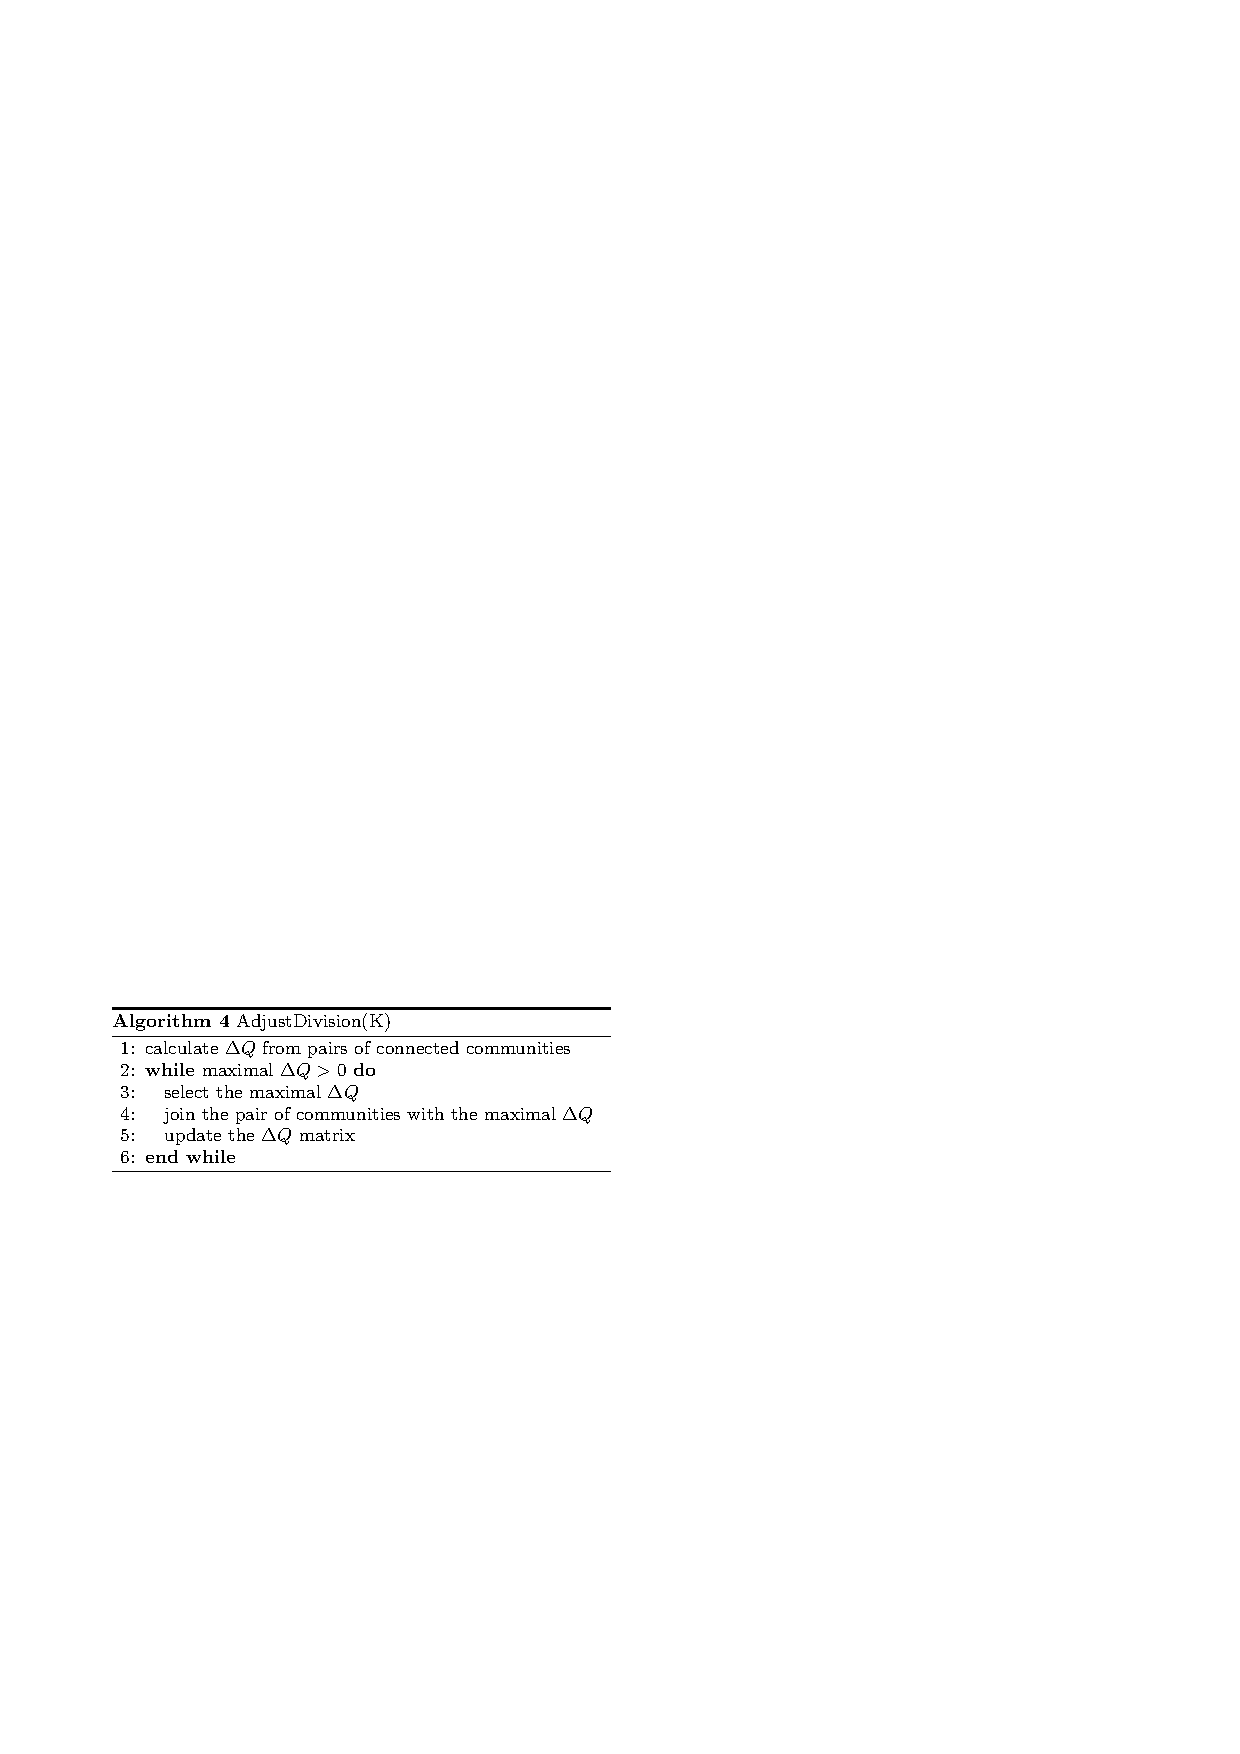
\includegraphics[height=4cm]{images/adjustDivision.pdf}
\end{center}
\end{frame}